\section{Berechnung}\label{sec:Berechnung}
In diesem Kapitel wird anhand der Abbildung \ref{fig:berechnung} die Abstände zwischen den Elementen sowie die Länge des Dipols, des Reflektor und der Direktoren berechnet. Die Yagi-Antenne soll für eine Frequenz von \SI{144.125}{MHz} ausgelegt werden. Diese Frequenz entspricht dem 2-Meter-Band, welches von den Funkamateuren für eine Erde-Mond-Erde-Übertragung benutzt wird.

\begin{figure}[H]
	\centering
	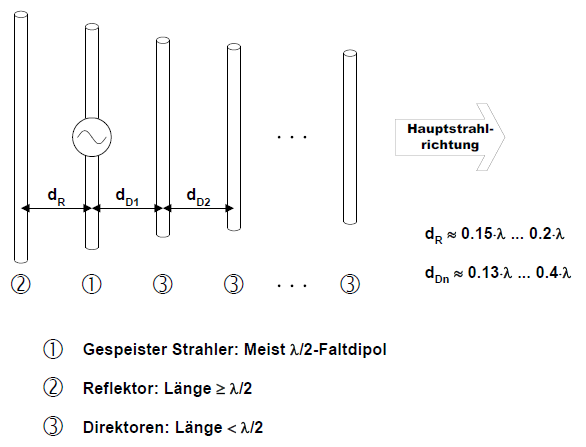
\includegraphics[width=0.9\linewidth]{yagi_berechnung}
	\caption{Aufbau einer Yagi-Antenne mit Dimensionsangaben \cite{script}.}\label{fig:berechnung}
\end{figure}

Die Antenne soll aus einem Reflektor, einem Dipol und fünf Direktoren bestehen. Die benötigten Elemente werden nachfolgend berechnet.

Die Wellenlänge $ \lambda $ für \SI{144.125}{MHz} berechnet sich wie folgt:
\begin{equation}
\lambda=\frac{c}{f_{0}}=\frac{\SI{300e06}{m/s}}{
\SI{144.125}{MHz}} = \SI{2.08}{m}
\end{equation}

Die Länge des Reflektors $ l_\mathrm{R} $ wird folgend berechnet:
\begin{equation}
l_\mathrm{R}\geq\frac{\lambda}{2}=\frac{\SI{2.08}{m}}{
	2} = \SI{1.04}{m} \Rightarrow \SI{1.2}{m}
\end{equation}

Die Länge des Dipols $ l_\mathrm{S} $ (Strahler) lässt sich wie folgend berechnen:
\begin{equation}
l_\mathrm{S}=\frac{\lambda}{2}=\frac{\SI{2.08}{m}}{
	2} = \SI{1.04}{m}
\end{equation}

Die Länge der Direktoren $ l_\mathrm{Dn} $ berechnet sich folgendermassen:
\begin{equation}
l_\mathrm{Dn}\leq\frac{\lambda}{2}=\frac{\SI{2.08}{m}}{
	2} = \SI{1.04}{m} \Rightarrow \SI{0.9}{m}
\end{equation}

Der Abstand $ d_\mathrm{R} $ zwischen Reflektor und Dipol berechnet sich wie folgt:
\begin{equation}
d_\mathrm{R}\approx 0.15\cdot\lambda=0.15\cdot \SI{2.08}{m}= \SI{0.312}{m}\Rightarrow \SI{0.32}{m}
\end{equation}

Der Abstand $ d_\mathrm{Dn} $ zwischen Dipol und Direktor oder Direktor und nachfolgendem Direktor wird berechnet mit:
\begin{equation}
d_\mathrm{Dn}\approx 0.2\cdot\lambda=0.2\cdot \SI{2.08}{m}= \SI{0.416}{m} \Rightarrow \SI{0.4}{m}
\end{equation}

Die Länge des Trägerstabes $ l_{T} $ wird folgend berechnet und beträgt minimal:
\begin{equation}
l_\mathrm{T}=d_\mathrm{R}+5\cdot d_\mathrm{Dn} + \mathrm{Anfang} = \SI{0.32}{m} + 5\cdot \SI{0.4}{m} + \SI{0.2}{m}= \SI{2.52}{m}
\end{equation}

Alle Masse sind in der Tabelle \ref{tab:bauwerte} zusammengefasst.

\begin{table}[H]
	\centering
	\begin{tabular}{>{\tt}L{6cm}|  L{3cm}}
		\normalfont\textbf{Name} 	& \normalfont\textbf{Masse [m]} \\ \hline\hline
		Wellenlänge $\lambda$		&  2.08    \\ \hline
		Länge Reflektor $ l_\mathrm{R} $	&  1.2    \\ \hline
		Länge Dipol $ l_\mathrm{S} $		&  1.04    \\ \hline
		Länge Direktor $ l_\mathrm{Dn} $ 	&  0.9     \\ \hline
		Länge Trägerstab $ d_\mathrm{T} $ 	&  2.52    \\ \hline
		Distanz $ d_\mathrm{R} $ 			&  0.32   \\ \hline
		Distanz $ d_\mathrm{Dn} $ 			&  0.4    \\ \hline
	\end{tabular}
	\caption{Zusammenstellung der Längen der Elemente sowie deren Abstand zueinander.}
	\label{tab:bauwerte}
\end{table}
